\documentclass{article}

\usepackage{graphicx}
\usepackage{tikz}
\usepackage{tikz-qtree}
\newcommand*\circled[1]{\tikz[baseline=(char.base)]{
            \node[shape=circle,draw,inner sep=2pt] (char) {#1};}}

\begin{document}
\title{Homework 18}
\date{}
\maketitle

% 1. Spring 2008 Final, #5
% 2. Fall 2011 Final, #8
% 3. Fall 2012 Final, #8
% 4. Textbook 5.2.3, 5.2.4

\paragraph{\Large 1. Spring 2008 Final Question 5}\mbox{}\\
Consider the following TST, where the black nodes correspond to strings in the TST.\\

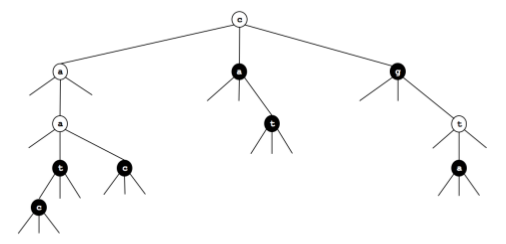
\includegraphics[]{fin-s08-5.png}\\
\begin{enumerate}
\renewcommand{\theenumi}{\Alph{enumi}}
	\item Which 7 strings (in alphabetical order) are in the TST?\\
	
	aac aat ac ca ct g ta  

	\item Draw the results of adding the following strings into the TST above:\\

	cgt \quad aaca \quad tt\\

	Results cut from solution pdf after first drawing the correct answer by hand.\\
	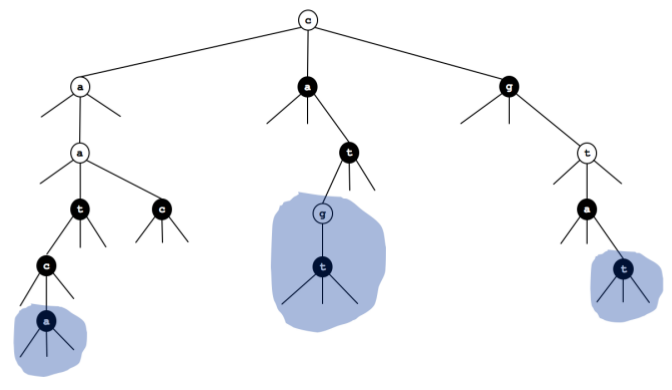
\includegraphics[width=\linewidth]{fin-s08-5b.png}

\end{enumerate}

\paragraph{\Large 2. Fall 2011 Final Question 8}\mbox{}\\
Consider the following ternary search trie, with string keys and integer values.\\

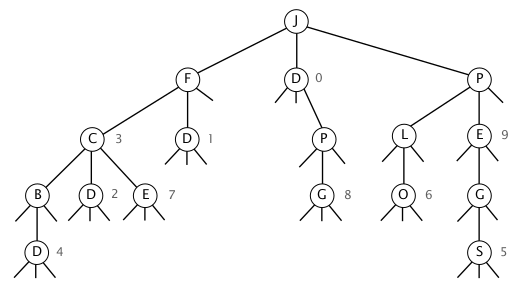
\includegraphics[]{fin-f11-8.png}\\

Circle which one or more of the following strings are keys in the TST.\\

B \quad \circled{BD} \quad \circled{C} \quad \circled{CD} \quad D \quad \circled{E} \quad \circled{FD} \quad JLO \quad JP \quad JPEG \quad JPEGS \quad \circled{JPG} \quad PEG \quad \circled{PEGS}\\

\paragraph{\Large 3. Fall 2012 Final Question 8}\mbox{}\\
Consider the following ternary search trie, where the values are shown next to the nodes of the corresponding string keys.\\

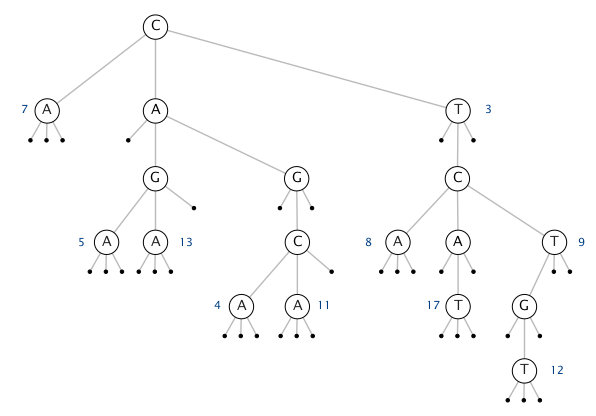
\includegraphics[]{fin-f12-8.png}\\

\begin{enumerate}
\renewcommand{\theenumi}{\Alph{enumi}}
	\item Circle which one or more of the following strings are keys in the TST?\\

	\circled{A} \quad AGA \quad CA \quad \circled{CAA} \quad CACA \quad CAT \quad \circled{CGA} \quad \circled{CGCA} \quad \circled{TA} \quad TC \quad TCA \quad \circled{TGT} \quad \circled{TT} \quad TTT

	\item Insert the two strings CGTT and TGA into the TST with the associated values 0 and 99, respectively; update the figure above to reflect the changes.

	Results cut from solution pdf after first drawing the correct answer by hand.\\
	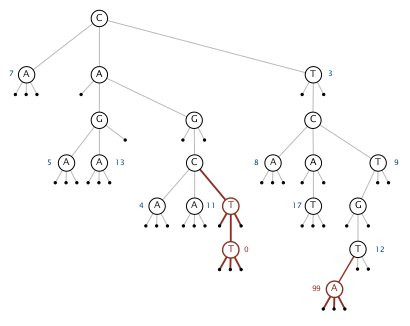
\includegraphics[width=\linewidth]{fin-f12-8b.png}

\end{enumerate}

\paragraph{\Large 4. Question 5.2.3 and 5.2.4}\mbox{}\\
Draw the $R$-way trie that results when the keys\\

now \quad is \quad the \quad time \quad for \quad all \quad good \quad people \quad to \quad come \quad to \quad the \quad aid \quad of\\

are inserted in that order into an initially empty trie (do not draw null links).\\

\Tree [
[.a [.i d ] [.l l ] ]
[.f [.o r ] ]
[.g [.o [.o d ] ] ]
[.i s ]
[.n [.o w ] ]
[.o f ]
[.p [.e [.o [.p [.l e ] ] ] ] ]
[.t [.h e ] [.i [.m e ] ] o ]
]\\

Draw the $R$-way trie that results when the keys\\

now \quad is \quad the \quad time \quad for \quad all \quad good \quad people \quad to \quad come \quad to \quad the \quad aid \quad of\\

are inserted in that order into an initially empty TST.\\

\Tree [.n 
[.i 
	[.f [.a [.c [.o [.m e ] ] ]
			[.l [.i [.d ] ] l ] ]
		[.o r ]
		[.g [.o [.o d ] ] ] ]
	s ]
[. o w ]
[.t
	[.p [.o f ]
		[.e [.o [.p l ] ] ] ] 
	[.h o e ]
	[.i [.m e ] ] ]
]

\end{document}